% Source: Lecture6.pdf, pages 1-7 (page 8 is blank).
\lecture{6}
\paragraph{1D Ising model, continued.}

Recall: with PBC,
$Z = \sum_{\{\sigma_i\}}e^{-\beta\Ham} = \Tr(T^N)$, where $T$ = transfer matrix, with
matrix elements
\begin{equation}
  \langle\sigma_{i+1}|T|\sigma_i\rangle = e^{K\sigma_{i+1}\sigma_i+(h/2)(\sigma_{i+1}+\sigma_i)},
  \qquad K\equiv\beta J,\quad h\equiv\beta H,
  \qquad
  T = \begin{pmatrix} e^{K+h} & e^{-K}\\ e^{-K} & e^{K-h}\end{pmatrix}.
\end{equation}
For $H = 0$, the eigenvalues of $T$ are $\lambda_+ = 2\cosh K$, $\lambda_- = 2\sinh K$. So
\begin{equation}
  Z = \Tr(T^N) = \lambda_+^N + \lambda_-^N = 2^N(\cosh K)^N[1+v^N],\qquad v = \tanh K .
\end{equation}
The Gibbs free energy per site is $\bar G(T,H) = -\kB Tf$, where $f$ = the dimensionless
reduced free energy. We will usually take the thermodynamic limit $N\to\infty$, with
\begin{equation}
  f = \lim_{N\to\infty}\frac{1}{N}\ln Z = \ln[2\cosh K] = \ln(\lambda_+).
\end{equation}
This illustrates that $f$ and the resultant thermodynamic functions are determined by the
dominant (= maximal) eigenvalue of the transfer matrix. This is $\lambda_+$ since
$\cosh K>\sinh K$. The internal energy per site is
\begin{equation}
  \bar U = -\pder{f}{\beta} = -J\pder{f}{K} = -J\tanh K = -J\tanh(\beta J).
\end{equation}
N.B.: this is invariant under $J\to -J$.

\subsubsection*{Ferromagnet--antiferromagnet mapping on bipartite lattices}

\paragraph{Theorem.} On a bipartite lattice,
$\Lambda = \Lambda_e\oplus\Lambda_o$, there is a mapping that relates a spin model with the
FM sign of $J$, $J>0$, to the model with the AFM sign of $J$, $J<0$, if the external field
$H = 0$. The mapping is
\begin{equation}
  J\to -J,\qquad
  \sigma_i\to\sigma_i\ \text{if } i\in\Lambda_e,\qquad
  \sigma_i\to-\sigma_i\ \text{if } i\in\Lambda_o .
\end{equation}
Then
$\Ham = -J\sum_{\langle ij\rangle}\sigma_i\sigma_j\to-(-J)\sum_{\langle ij\rangle}(-\sigma_i\sigma_j)$
is invariant, since all of the nearest neighbors of a site $i\in\Lambda_{\text{even}}$ are
in $\Lambda_{\text{odd}}$.

\begin{diagram}
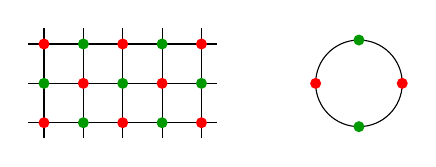
\begin{tikzpicture}[scale=0.5]
  \foreach \x in {0,...,4} \draw (\x,-0.4) -- (\x,2.4);
  \foreach \y in {0,1,2} \draw (-0.4,\y) -- (4.4,\y);
  \foreach \x in {0,...,4} \foreach \y in {0,1,2} {
    \pgfmathtruncatemacro{\prty}{mod(\x+\y,2)}
    \ifnum\prty=0 \fill[red] (\x,\y) circle (0.14); \else \fill[green!60!black] (\x,\y) circle (0.14); \fi}
  \begin{scope}[xshift=8cm,yshift=1cm]
    \draw (0,0) circle (1.1);
    \fill[green!60!black] (0,1.1) circle (0.14); \fill[green!60!black] (0,-1.1) circle (0.14);
    \fill[red] (1.1,0) circle (0.14); \fill[red] (-1.1,0) circle (0.14);
  \end{scope}
\end{tikzpicture}
\diagramcaption{Bipartite lattices: each red site has nearest neighbors that are green,
and vice versa. Left: the square lattice. Right: a 1D ring with an even number of sites.}
\end{diagram}

Our 1D lattice is bipartite iff $N$ is even, and we can take the limit $N\to\infty$ on even
values. The interaction Hamiltonian is invariant under this mapping, and so is the sum
$\sum_{\{\sigma_i\}}e^{-\beta\Ham}$, since each $\sigma_i$ takes on $\pm 1$ values. So for the
$H = 0$ case we can, with no loss of generality, take $J>0$:
\begin{equation}
  \bar U = -J\ev{\sigma_2\sigma_1} = -J\tanh(\beta J).
\end{equation}
As $T\to\infty$, $\beta\to 0$, the spins are random, so $\ev{\sigma_2\sigma_1}\to 0$. As
$T\to 0$, the FM coupling favors short-range order; $\tanh(\beta J)\to 1$ as $\beta\to\infty$.
(See the plot of $\bar U$ at the end of the previous lecture.)

\subsubsection*{Specific heat of the 1D Ising model}

Next, calculate the specific heat (per spin), $\bar C = \left.\dd\bar U/\dd T\right|_{H=0}$;
we drop the bars in the notation henceforth. Now
$K = \beta J = J/(\kB T)$, i.e.\ $T = J/(\kB K)$, so $\dd T = -(J/(\kB K^2))\dd K$, i.e.\
$\dd K/\dd T = -\kB K^2/J$. With $U = -\partial f/\partial \beta = -J\partial f/\partial K$,
\begin{equation}
  C = \pder{U}{T} = \pder{K}{T}\cdot\pder{U}{K}
    = \left(-\frac{\kB K^2}{J}\right)\pder{U}{K}
    = -\left(\frac{\kB K^2}{J}\right)\pder{}{K}\left(-J\pder{f}{K}\right)
    = \kB K^2\frac{\partial^2 f}{\partial K^2}.
\end{equation}
($C$ is the second derivative of $f$ with respect to $T$, or equivalently $K$.) Since
$(\dd/\dd K)\tanh K = 1/(\cosh^2K)$,
\begin{equation}
  C = \left(-\frac{\kB K^2}{J}\right)\left(-\frac{J}{\cosh^2K}\right) = \frac{\kB K^2}{\cosh^2K}.
\end{equation}
Now $\cosh K = (e^K+e^{-K})/2$, so as
\begin{equation}
  \begin{cases}
    T\to\infty,\ \text{i.e.}\ \beta\to 0,\ K\to 0: & \cosh K\to 1,\\[6pt]
    T\to 0,\ \text{i.e.}\ \beta\to\infty,\ K\to\infty: & \cosh K\sim\dfrac{e^K}{2}.
  \end{cases}
\end{equation}
So as $T\to 0$, $C\to 4\kB K^2e^{-2K}\propto 4\kB T^{-2}e^{-2J/T}$, an essential zero; as
$T\to\infty$, $C\to\kB K^2\propto T^{-2}$, which vanishes as a power of $T$.

\begin{diagram}
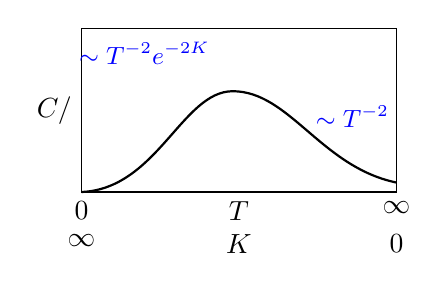
\begin{tikzpicture}[scale=0.8]
  \draw (0,0) rectangle (5,2.6);
  \draw[thick] (0,0) .. controls (1.2,0.05) and (1.6,1.6) .. (2.4,1.6) .. controls (3.3,1.6) and (3.8,0.4) .. (5,0.15);
  \node[left] at (0,1.3) {$C/\kB$};
  \node[below] at (0,0) {$0$}; \node[below] at (5,0) {$\infty$}; \node[below] at (2.5,0) {$T$};
  \node[below=12pt] at (0,0) {$\infty$}; \node[below=12pt] at (5,0) {$0$}; \node[below=12pt] at (2.5,0) {$K$};
  \node[blue,font=\small] at (1,2.2) {$\sim T^{-2}e^{-2K}$};
  \node[blue,font=\small] at (4.3,1.2) {$\sim T^{-2}$};
\end{tikzpicture}
\diagramcaption{Schematic graph of the specific heat of the 1D Ising model.}
\end{diagram}

This behavior can be understood physically: the specific heat $C$ measures how the internal
energy changes as one changes the temperature $T$. As $T\to 0$, the spins are approaching a
frozen state $+++++$ or $-----$, and $U$ approaches $-J$, so taking $T\to 0.1\,T$ has almost
no effect, so $C\to 0$. As $T\to\infty$, the spins are almost completely random, and
$U\to 0$, so taking $T\to 10\,T$ has a negligible effect on $U$ and hence again, $C\to 0$. The
specific heat reaches a max at an intermediate temperature $T$ such that $\kB T\sim J$, since
for temperatures of this order a change in $T$ has a significant effect on the local spin
order and hence on $U$.

\subsection{The 1D Ising model in a magnetic field}
\subsubsection*{Nonzero external field}

Next, apply a nonzero external magnetic field $H$. Calculate the eigenvalues of the transfer
matrix $T$. Recall
$T = \left(\begin{smallmatrix} e^{K+h} & e^{-K}\\ e^{-K} & e^{K-h}\end{smallmatrix}\right)$.
The indicial equation for the eigenvalues is
\begin{gather}
  (e^{K+h}-\lambda)(e^{K-h}-\lambda) - e^{-2K} = 0\nonumber\\
  \Rightarrow\ \lambda^2 - (e^{K+h}+e^{K-h})\lambda + (e^{2K}-e^{-2K}) = 0
  \ \Rightarrow\ \lambda^2 - e^K\,2\cosh h\,\lambda + 2\sinh(2K) = 0,
\end{gather}
so
\begin{align}
  \lambda_\pm &= \frac{1}{2}\left[2e^K\cosh h\pm\sqrt{4e^{2K}\cosh^2h - 8\sinh(2K)}\right]\nonumber\\
  &= e^K\left[\cosh h\pm\sqrt{\cosh^2h - 2e^{-2K}\sinh(2K)}\right]\nonumber\\
  &= e^K\left[\cosh h\pm\sqrt{\left(\frac{e^h+e^{-h}}{2}\right)^2 - 2e^{-2K}\left(\frac{e^{2K}-e^{-2K}}{2}\right)}\right]\nonumber\\
  &= e^K\left[\cosh h\pm\sqrt{\frac{1}{4}(e^{2h}+2+e^{-2h}) + (-1+e^{-4K})}\right].
\end{align}
Since $(1/4)(e^{2h}+2-4+e^{-2h}) = (\sinh h)^2$, an equivalent expression for $\lambda_\pm$
is
\begin{equation}
  \lambda_\pm = e^K\left[\cosh h\pm\sqrt{(\sinh h)^2+e^{-4K}}\right],\qquad h = \beta H .
\end{equation}
Here $\lambda_+$ is the maximal eigenvalue of $T$, and $f = \ln\lambda_+$,
$\bar G(T,H) = -\kB Tf = -\beta^{-1}f$.

\paragraph{Magnetization.}

Now calculate the induced magnetization per site:
\begin{equation}
  \bar M = \lim_{N\to\infty}\frac{1}{N}\left[\frac{\sum_{\{\sigma_i\}}\left(\sum_j\sigma_j\right)e^{-\beta\Ham}}{\sum_{\{\sigma_i\}}e^{-\beta\Ham}}\right]
  = \left(\pder{f}{h}\right)_T = \frac{1}{\beta}\left(\pder{f}{H}\right)_T = -\left(\pder{\bar G}{H}\right)_T ;
\end{equation}
recall $\dd G(T,H) = -S\dd T - M\dd H$, so $M = -(\partial G/\partial H)_T$. So
\begin{equation}
  \bar M = \pder{\ln\lambda_+}{h} = \frac{1}{\lambda_+}\pder{\lambda_+}{h};
  \qquad\text{define}\quad \tilde\lambda_+ = e^{-K}\lambda_+ .
\end{equation}
Now
\begin{equation}
  \pder{\tilde\lambda_+}{h} = \sinh h + \frac{1}{2}\cdot\frac{2(\sinh h)(\cosh h)}{\sqrt{\sinh^2h+e^{-4K}}}
  = (\sinh h)\left[1 + \frac{\cosh h}{\sqrt{\sinh^2h+e^{-4K}}}\right],
\end{equation}
\begin{equation}
  \frac{1}{\lambda_+}\pder{\lambda_+}{h} = \frac{1}{\tilde\lambda_+}\pder{\tilde\lambda_+}{h}
  = \frac{(\sinh h)\left[\frac{\sqrt{\sinh^2h+e^{-4K}}+\cosh h}{\sqrt{\sinh^2h+e^{-4K}}}\right]}{\cosh h+\sqrt{\sinh^2h+e^{-4K}}}
  = \frac{\sinh h}{\sqrt{\sinh^2h+e^{-4K}}},
\end{equation}
so
\begin{equation}
  \boxed{\bar M = \frac{\sinh h}{\sqrt{\sinh^2h+e^{-4K}}}}\,;
  \qquad\text{spontaneous magnetization}\quad \bar M_{\text{spont.}} = \lim_{h\to 0}\bar M .
\end{equation}
For any temperature $T>0$, hence finite $K = \beta J$, this limit $=0$:
$\bar M_{sp} = 0\ \forall\, T>0$. If we set $T = 0$, i.e.\ $\beta = \infty$, $K = \infty$, then
$e^{-4K} = 0$, so $|\bar M| = 1$ ($\bar M = \sgn(H)$). So
\begin{equation}
  |\bar M| = \begin{cases} 0 & \forall\, T>0\\ 1 & \text{for } T = 0.\end{cases}
\end{equation}
$\bar M_{sp}$ thus has a discontinuous behavior as $T\to 0$.

\begin{diagram}
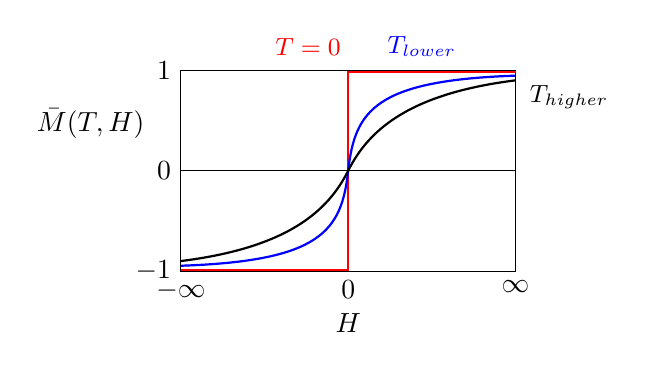
\begin{tikzpicture}[scale=0.85]
  \draw (0,0) rectangle (5,3);
  \draw (0,1.5) -- (5,1.5); \draw (2.5,0) -- (2.5,3);
  \draw[thick,red] (0,0.02) -- (2.5,0.02) -- (2.5,2.98) -- (5,2.98);
  \draw[thick,blue] (0,0.08) .. controls (2.1,0.15) and (2.4,0.6) .. (2.5,1.5) .. controls (2.6,2.4) and (2.9,2.85) .. (5,2.92);
  \draw[thick] (0,0.15) .. controls (1.6,0.35) and (2.2,0.9) .. (2.5,1.5) .. controls (2.8,2.1) and (3.4,2.65) .. (5,2.85);
  \node[left] at (0,3) {$1$}; \node[left] at (0,1.5) {$0$}; \node[left] at (0,0) {$-1$};
  \node[left] at (-0.4,2.2) {$\bar M(T,H)$};
  \node[below] at (0,0) {$-\infty$}; \node[below] at (2.5,0) {$0$}; \node[below] at (5,0) {$\infty$};
  \node[below=12pt] at (2.5,0) {$H$};
  \node[red,font=\small] at (1.9,3.35) {$T=0$};
  \node[blue,font=\small] at (3.6,3.35) {$T_{\text{lower}}$};
  \node[font=\small] at (5.8,2.6) {$T_{\text{higher}}$};
\end{tikzpicture}
\diagramcaption{Magnetization of the 1D Ising model, taking account of the reversal in
$\sgn(\bar M)$ with $\sgn(H)$.}
\end{diagram}

\subsubsection*{The Peierls theorem in one dimension}

The fact that there is no spontaneous magnetization, i.e.\ no ``long-range order'' (LRO), at
any finite temperature in this model is a consequence of a general theorem, the (1D form of
the) \emph{Peierls theorem}: given a spin system with finite-range interactions (e.g.\
nearest-neighbor interactions), there is no LRO = spontaneous magnetization at any $T>0$.

\paragraph{Proof.} The equilibrium state is obtained by minimizing the free energy. Consider
$A = U - TS$ (or $G = U - TS - HM$, with $H = 0$). Consider a hypothetical ordered state
$+++++\cdots$ and show that it is unstable to the appearance of a seam (for FBC) with reversal
of spins: $+++++\,|\,-----$. The change in $\Delta A$ or $\Delta G$ is
\begin{equation}
  \Delta G = +2J - T\ln N,
\end{equation}
where the bond energy changes from $-J$ ($++$) to $+J$ ($+-$), a difference of $2J$, and
$-T\Delta S = -T\ln N$ since the seam can occur at any of the $N$ sites on the lattice. So
for any $T>0$, as $N\to\infty$, the entropy term dominates and $\Delta G<0$, so the disordering
seams are preferred over the hypothetical ordered state. Only at $T = 0$ is the entropy term
absent; then $\Delta G = \Delta U$ and the appearance of the seam is dispreferred. That is,
if and only if $T = 0$, then the minimization of the free energy is the same as the
minimization of the internal energy.

\subsubsection*{Susceptibility}

Next, calculate the (isothermal) magnetic susceptibility $\chi = (\partial M/\partial H)_T$
and, per site,
\begin{equation}
  \bar\chi = \left(\pder{\bar M}{H}\right)_T = \beta\left(\pder{\bar M}{h}\right)_T
  = \beta\left(\frac{\partial^2 f}{\partial h^2}\right)_T .
\end{equation}
As is evident, $\chi$ is a second derivative of $f$ with respect to $h$. Now
\begin{align}
  \pder{\bar M}{h} &= \pder{}{h}\left[\frac{\sinh h}{\sqrt{\sinh^2h+e^{-4K}}}\right]\nonumber\\
  &= \frac{\cosh h}{\sqrt{\sinh^2h+e^{-4K}}}
    - \frac{1}{2}(\sinh h)(\sinh^2h+e^{-4K})^{-3/2}\cdot(2\sinh h\cosh h)\nonumber\\
  &= \frac{\cosh h}{\sqrt{\sinh^2h+e^{-4K}}}\left[1-\frac{\sinh^2h}{\sinh^2h+e^{-4K}}\right]
   = \frac{e^{-4K}\cosh h}{(\sinh^2h+e^{-4K})^{3/2}},
\end{align}
so
\begin{equation}
  \bar\chi = \frac{\beta e^{-4K}\cosh h}{(\sinh^2h+e^{-4K})^{3/2}};
  \qquad\text{zero-field susceptibility:}\quad \bar\chi_{H=0} = \beta e^{2K}.
\end{equation}
$\bar\chi_{H=0}$ diverges exponentially as $T\to 0$, i.e.\ $K\to\infty$ (an essential divergence
$\sim e^{2J/T}$ as a function of $T$). So the 1D Ising model has a (1-sided) phase transition at
$T = 0$. Rather than algebraic singularities, it has a combination of essential singularities in
$\bar C$ and $\bar\chi_{H=0}$ and a discontinuous singularity in
$M_{H=0} = M_{\text{spontaneous}}$.

\subsection{Correlations in the 1D Ising model}
\subsubsection*{Spin--spin correlation function by a high-temperature expansion}

Calculate the spin--spin correlation function
$\ev{\sigma_i\sigma_j}_{H=0} = \ev{\sigma_i\sigma_j}_{\text{conn.},H=0}$, where $i$, $j$ are
arbitrary. The method is a high-temperature series expansion. Here
\begin{equation}
  \ev{\sigma_i\sigma_j}_{\text{conn}}\equiv\ev{\sigma_i\sigma_j}-\ev{\sigma}^2 = \ev{\sigma_i\sigma_j}-\bar M^2 .
\end{equation}
Consider $T>0$; here $\bar M = 0$, so $\ev{\sigma_i\sigma_j} = \ev{\sigma_i\sigma_j}_{\text{connected}}$.
With $\langle ij\rangle$ the nearest neighbors (n.n.),
\begin{equation}
  Z = \sum_{\{\sigma_i\}}e^{-\beta\Ham} = \sum_{\{\sigma_i\}}e^{K\sum_{\langle ij\rangle}\sigma_i\sigma_j}
    = \sum_{\{\sigma_i\}}\left[\prod_{\langle ij\rangle}e^{K\sigma_i\sigma_j}\right].
\end{equation}
Use $e^x = \sum_{n=0}^\infty x^n/n!$ and $\sigma_i = \pm 1$, $\sigma_i^2 = 1$:
\begin{align}
  e^{K\sigma_i\sigma_j} &= 1 + K\sigma_i\sigma_j + \frac{1}{2!}(K\sigma_i\sigma_j)^2
     + \frac{1}{3!}(K\sigma_i\sigma_j)^3 + \frac{1}{4!}K^4 + \frac{1}{5!}K^5\sigma_i\sigma_j+\cdots\nonumber\\
  &= \underbrace{\left[1+\frac{K^2}{2!}+\frac{K^4}{4!}+\cdots\right]}_{\cosh K}
   + \sigma_i\sigma_j\underbrace{\left[K+\frac{K^3}{3!}+\frac{K^5}{5!}+\cdots\right]}_{\sinh K}
\end{align}
(recall $\cosh x = 1 + x^2/2!+x^4/4!+\cdots$ and
$\sinh x = x + x^3/3!+x^5/5!+\cdots$), so
\begin{equation}
  e^{K\sigma_i\sigma_j} = \cosh K + \sigma_i\sigma_j\sinh K = \cosh K\,(1+v\sigma_i\sigma_j),
  \qquad v\equiv\tanh K .
\end{equation}
This is an identity; $|v|\to 0$ as $T\to\infty$. Therefore
\begin{equation}
  Z = \sum_{\{\sigma_i\}}\left[\prod_{\langle ij\rangle}e^{K\sigma_i\sigma_j}\right]
    = \sum_{\{\sigma_i\}}\prod_{\langle ij\rangle}\cosh K\,(1+v\sigma_i\sigma_j)
    = (\cosh K)^{e(\Lambda)}\sum_{\{\sigma_i\}}\left[\prod_{\langle ij\rangle}(1+v\sigma_i\sigma_j)\right],
\end{equation}
since to each n.n.\ pair $\langle ij\rangle$ there is a bond. For a lattice $\Lambda$ with
coordination number $\Delta\equiv$ degree of each site in $\Lambda$,
\begin{equation}
  e(\Lambda) = \frac{\Delta}{2}n(\Lambda),
\end{equation}
so $e(\Lambda_{1D}) = n$ for a 1D lattice with PBC, and
\begin{equation}
  Z = (\cosh K)^{(\Delta/2)n}\sum_{\{\sigma_i\}}\left[\prod_{\langle ij\rangle}(1+v\sigma_i\sigma_j)\right].
\end{equation}

\paragraph{Example: a triangle.} Illustrate this with a calculation of $Z$ for a (finite)
$\Lambda$, the triangle with vertices 1, 2, 3:
\begin{align}
  Z &= (\cosh K)^3\sum_{\{\sigma_i\}}(1+v\sigma_1\sigma_2)(1+v\sigma_2\sigma_3)(1+v\sigma_3\sigma_1)\nonumber\\
    &= (\cosh K)^3\sum_{\{\sigma_i\}}\left[1 + v(\sigma_1\sigma_2+\sigma_2\sigma_3+\sigma_3\sigma_1)
       + v^2(\sigma_1\sigma_2\sigma_2\sigma_3+\text{cycl.}) + v^3\sigma_1\sigma_2\sigma_2\sigma_3\sigma_3\sigma_1\right]\nonumber\\
    &= (\cosh K)^3(1+v^3)\cdot 2^3 ,
\end{align}
since the terms linear in $v$ and the terms $v^2\sigma_1\sigma_3$ etc.\ sum to zero. So for this
illustrative example with $N = 3$,
\begin{equation}
  Z = (2^3)(\cosh K)^3(1+v^3) = (2\cosh K)^3 + (2\sinh K)^3 = \lambda_+^N+\lambda_-^N\quad\text{with } N = 3 .
\end{equation}
This shows how this expansion yields $Z$ and shows the method (series in powers of $K$, or
equivalently $v$) used in high-temperature series.

\paragraph{Correlation function.} Now use this method to calculate $\ev{\sigma_n\sigma_{n'}}$.
Note that, due to the homogeneity of $\Lambda$ (with PBC), this 2-spin correlation function
only depends on $|n-n'|$. E.g.\ calculate $\ev{\sigma_0\sigma_2}$ on a ring of sites
$0,1,2,3$:
\begin{equation}
  \ev{\sigma_0\sigma_2} = \frac{\sum_{\{\sigma_i\}}\sigma_0\sigma_2e^{-\beta\Ham}}{\sum_{\{\sigma_i\}}e^{-\beta\Ham}}
  = \frac{\sum_{\{\sigma_i\}}\sigma_0\sigma_2\prod_{\langle ij\rangle}(1+v\sigma_i\sigma_j)}{\sum_{\{\sigma_i\}}\prod_{\langle ij\rangle}(1+v\sigma_i\sigma_j)}.
\end{equation}
The numerator is
\begin{align}
  &\sum_{\{\sigma_i\}}\sigma_0\sigma_2(1+v\sigma_0\sigma_1)(1+v\sigma_1\sigma_2)(1+v\sigma_2\sigma_3)(1+v\sigma_3\sigma_0)\nonumber\\
  &\quad= \sum_{\{\sigma_i\}}\sigma_0\sigma_2\left[1 + v(\sigma_0\sigma_1+\text{cycl.}) + v^2(\sigma_0\sigma_1\cdot\sigma_1\sigma_2+\cdots)+\cdots\right]
  \ \propto\ v^2 + v^{N-2}
\end{align}
(any unmatched $\sigma_i$ gives zero after the sum). Now generalize this; by a similar method,
\begin{equation}
  \ev{\sigma_0\sigma_\ell} = v^\ell + v^{N-\ell}.
\end{equation}
Next, take the thermodynamic limit $N\to\infty$. For our $T>0$ regime, $|v|<1$, so
$\lim_{N\to\infty}v^{N-\ell} = 0$ and hence
\begin{equation}
  \boxed{\ev{\sigma_0\sigma_\ell} = v^\ell},\qquad v = \tanh K .
\end{equation}
This completes the calculation of the 2-spin correlation function in the 1D Ising model
(for $H = 0$).
